\chapter{設計と実装}
本章では,提案ツールおよび提案ツールを動作するシミュレータについて述べる.

\section{開発環境}
提案ツールの開発環境を下記に示す.

\begin{itemize}
    \item OS:macOS Big Sur 11.1
    \item プログラミング言語:Python 3.7
    \item 統合開発環境:PyCharm 2020.3.2
\end{itemize}

\section{提案ツールのアーキテクチャ}
\label{toolartchitecture}

\begin{figure}[H]
    \centering
    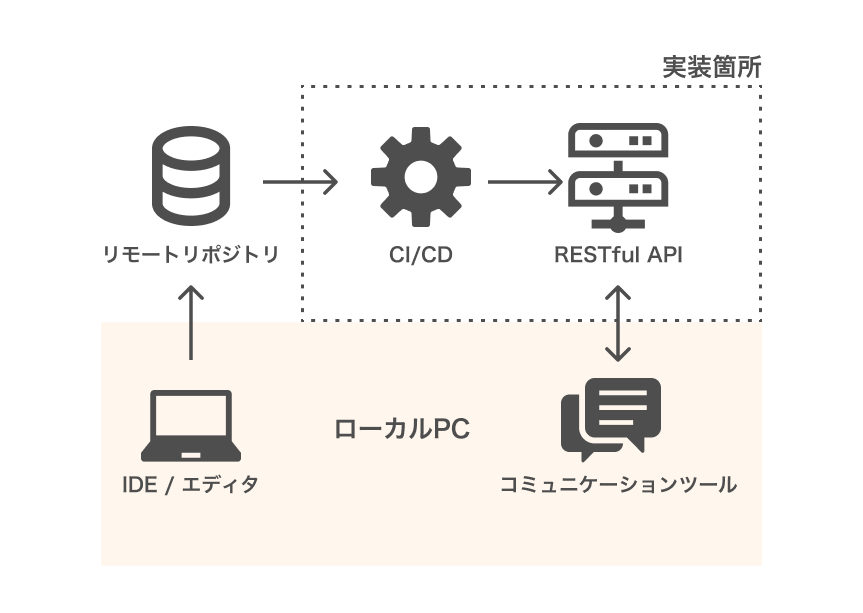
\includegraphics[width=12cm]{images/architecture.png}
    \caption{提案ツールのアーキテクチャ}
    \label{architecture}
\end{figure}

提案ツールのアーキテクチャを図\ref{architecture}に示す.
提案ツールは,既存のCI/CDツール上で動作することを想定しており,本研究ではCI/CDツールにGitHub Actions\cite{actions}を用いた.
また,CI/CDツール上で乖離の検知を行うが,できることが限られているため,同時に,Slackとのやりとりや,開発プロジェクトの状態の管理を行うことができるRESTful APIの開発も行った.
RESTful APIにはFastAPIを使用し,各種データの保持はJSONファイルにて管理を行っている.
また,RESTful APIは筆者のローカルPC上で動作させているが,HTTPSとして外部公開させることができるツールのngrok\cite{ngrok}を使用しており,
Slack APIやCI/CDツール上で動作する提案ツールは,ローカルPC上で動作するRESTful APIを使用できるようになっている.
加えて,提案ツールを利用するためには,CI/CDツールの設定ファイルに数行追加するだけでよく,非常に軽量であると言える.

Slackからに入力したコマンドをRESTful APIに反映させるための手順を下記にまとめる.
\begin{enumerate}
    \item Slackにコマンドを入力する
    \item Incoming Webhookより,SlackからRESTful APIに入力したコマンド内容がPOSTで送信される
    \item RESTful APIでは,受け取ったコマンドを解析し,適切な処理を行う
    \item 必要があれば,Slackにメッセージを送信する
\end{enumerate}

また,乖離検知を行い,検知した内容をSlackへと送信するための手順を下記にまとめる.
\begin{enumerate}
    \item GitHubへのプッシュを検知し,CI/CDツールが起動する
    \item CI/CDツール上で乖離検知を行うために,必要なデータをRESTful APIから取得する
    \item 取得したデータをもとに,乖離検知を行う
    \item 乖離検知をした場合,検知した内容を整形してメッセージとしてまとめ,RESTful APIにPOSTリクエストを行う
    \item RESTful APIからSlackにメッセージを送信する
\end{enumerate}

\section{RESTful APIの実装}
RESTful APIで利用可能な機能を下記にまとめる.
これらの機能はすべて1つのファイル(main.py)に集約されており,行数は202行である.
\begin{description}
    \item[GET:/data/\{project\_code\}] 乖離検知に必要なデータを取得
    \item[POST:/status/update/\{project\_code\}]  乖離検知に必要なデータを更新
    \item[GET:/git/log/\{project\_code\}] 整形したGitのコミット履歴を取得
    \item[POST:/git/log/\{project\_code\}] 整形したGitのコミット履歴を登録
    \item[POST:/message/\{project\_code\}] Slackに通知を送信
    \item[POST:/milk] Slackに入力したコマンドを受け取り,適切な処理を実行
\end{description}

また,RESTful APIに使用したライブラリとその選定理由を下記にまとめる.
\begin{description}
    \item[FastAPI] RESTful APIを簡易的に構築可能
    \item[Uvicorn] FastAPIを動作させるために必要
    \item[Slack Bolt] Slack APIとの通信を簡易的に行うことができる
    \item[requests] HTTPリクエストを直感的に扱うことが可能
\end{description}

\ref{toolartchitecture}節で述べたとおり,RESTful APIでは乖離検知に必要な状態管理を行っている.
下記に実際に提案ツールで使用している状態とパラメータの管理を行うJSONファイルの中身を示す.
パラメータはSlackからのコマンドによって更新され,状態はCI/CDツール上で動作するプログラムによって更新される.
例えば,C4のソースコード変更量の検知では,前回のドキュメントが更新されてから現在のソースコードの変更量が137行であることを示している.
\begin{lstlisting}[caption=状態とパラメメータの管理の例, label=status]
{
    "c1": {
        "param": {
            "code_type": ".py",
            "doc_file": "swagger.json"
        },
        "status": {}
    },
    "c2": {
        "param": {
            "doc_type": ".py",
            "code_type": ".md",
            "max_days": 7
        },
        "status": {
            "date": "2020-12-13"
        }
    },
    "c3": {
        "param": {
            "doc_type": ".py",
            "code_type": ".md",
            "path": "../../setup.py"
        },
        "status": {
            "version": "0.0.1"
        }
    },
    "c4": {
        "param": {
            "doc_type": ".py",
            "code_type": ".md"
        },
        "status": {
            "sum_change": 137,
            "max_change": 10000
        }
    }
}
\end{lstlisting}
    

\section{提案ツールの使用方法}
開発者は,適切なタイミングで変更を記録するためにコミットを実行し,リモートリポジトリにプッシュすることを期待している.
\ref{toolartchitecture}節にまとめたとおり,提案ツールはリモートリポジトリにプッシュされたタイミングで,CI/CDツールが起動し,CI/CDツールの設定ファイルに定義されたコマンドに従って実行される.
そのため,提案ツールはGitHub Actionsを利用可能な状況ではローカルPCに専用の環境を構築せずに利用することができる.
ただし,提案ツールを利用するにあたっていくつか準備が必要であるため,それについてまとめる.
まず,CI/CDツール上で動作させるために,プロジェクトのディレクトリにtoolsディレクトリを作成し,そのディレクトリの中にPythonで作成された提案ツールを配置する.
CI/CDツールの設定ファイルには,プッシュ時に提案ツールを実行するように記述するだけでよい.
次に,SlackのAPIページより,提案ツールを登録する必要がある.
最後にRESTful APIの動作環境を用意する必要がある.例えばGCP(Google Cloud Platform)\cite{gcp}やHeroku\cite{heroku}などのPaaS(Platform as aa Service)を利用することで,RESTful APIを動作する環境を用意することができる.
筆者が作成したRESTful APIをSaaSとして展開し,数多くのプロジェクトで利用することもできるが,現状ではセキュリティ上の懸念から各プロジェクトでRESTful APIを構築するのが望ましい.
いずれも,各Webサービスの登録手順に従って進めていくだけでよく,PaaSをよく理解していればRESTful APIの実行環境を簡単に構築することができる.

\section{コミュニケーションツールで利用可能なコマンド}
milkでは,Slackのスラッシュコマンドを活用することで,各種パラメータの設定を行うことができるようになっている.
以下では,milkで使用可能なコマンドをまとめる.

\subsection*{/milk c1 doc [ file type ]}
ソースコード先行検知の機能において,開発プロジェクトで使用するSwaggerドキュメントのファイル形式を指定することができるコマンドである.
本コマンドは,開発プロジェクトの初期段階でSwaggerドキュメントのファイル形式を指定する場合や,開発プロジェクトの途中でファイル形式を変更したい場合に利用されることを想定している.

\subsection*{/milk c1 code [ file type ]}
ソースコード先行検知の機能において,開発プロジェクトで使用するプログラミング言語を指定することができるコマンドである.
現在では,プログラミング言語にPythonのみを指定可能である.

\subsection*{/milk c1 param}
ソースコード先行検知の機能において,現在設定しているSwaggerドキュメントの拡張子および使用しているプログラミング言語の拡張子を確認することができるコマンドである.

\subsection*{/milk c2 set [ days ]}
一定時間経過後のリマインダーの機能において,ドキュメントが更新されずソースコードのみが更新されている場合に,ドキュメントを追加・修正するためのリマインダーを行う間隔を指定することができるコマンドである.

\subsection*{/milk c2 doc [ file type ]}
一定時間経過後のリマインダーの機能において,開発プロジェクトで使用するドキュメントのファイル形式を指定することができるコマンドである.
C2で使用するドキュメントは自由に指定可能である.

\subsection*{/milk c2 code [ file type ]}
一定時間経過後のリマインダーの機能において,開発プロジェクトで使用するプログラミング言語を指定することができるコマンドである.
C2で使用するプログラミング言語は自由に指定可能である.

\subsection*{/milk c2 param}
一定時間経過後のリマインダーの機能において,現在設定しているリマインダーを行う間隔やドキュメント,ソースコードの拡張子を確認することができるコマンドである.

\subsection*{/milk c3 set [ version file ]}
リリース時ドキュメント更新有無の検知の機能において,バージョンを扱うファイルを指定することができるコマンドである.
例えば,Pythonではsetup.pyと呼ばれるファイルにソフトウェアのバージョンを記述している.
現在では,バージョンを扱うファイルにsetup.pyのみを指定可能である.

\subsection*{/milk c3 doc [ file type ]}
リリース時ドキュメント更新有無の検知の機能において,開発プロジェクトで使用するドキュメントのファイル形式を指定することができるコマンドである.
C3で使用するドキュメントは自由に指定可能である.

\subsection*{/milk c3 code [ file type ]}
リリース時ドキュメント更新有無の検知の機能において,開発プロジェクトで使用するプログラミング言語を指定することができるコマンドである.
C3で使用するプログラミング言語は自由に指定可能である.

\subsection*{/milk c3 param}
リリース時ドキュメント更新有無の検知の機能において,現在設定しているバージョンを扱うファイルやドキュメント,ソースコードの拡張子を確認することができるコマンドである.

\subsection*{/milk c4 set [ number ]}
ソースコード変更量の検知の機能において,ドキュメントが更新されずソースコードのみが更新されている場合に,ソースコードの追加・削除・修正が行われた行数を指定することができるコマンドである.
指定した行数を超過してソースコードのみを記述し続けたときに通知がでる.

\subsection*{/milk c4 doc [ file type ]}
ソースコード変更量の検知の機能において,開発プロジェクトで使用するドキュメントのファイル形式を指定することができるコマンドである.
C4で使用するドキュメントは自由に指定可能である.

\subsection*{/milk c4 code [ file type ]}
ソースコード変更量の検知の機能において,開発プロジェクトで使用するプログラミング言語を指定することができるコマンドである.
C4で使用するプログラミング言語は自由に指定可能である.

\subsection*{/milk c4 param}
ソースコード変更量の検知の機能において,現在設定している変更量やドキュメント,ソースコードの拡張子を確認することができるコマンドである.

\section{シミュレータの設計}
シミュレーションには,CI/CDツール上で動作する乖離検知機能の一部を利用した.
シミュレーションの実行結果をグラフに描画するにあたり,Pythonのグラフ描画ライブラリであるMatplotlibを使用した.
以下に,シミュレーションを行う流れを示す.
\begin{enumerate}
    \item シミュレーションを行いたいリポジトリからGitコマンドを使用してコミット履歴を指定件数取得する
    \item 取得した文字列のコミット履歴を扱いやすいようにリストに整形する
    \item コミットごとにC1〜C4の機能を検証し,乖離リスクを検知したときに記録する
    \item 記録したデータをもとに,Matplotlibでグラフの描画を行う
\end{enumerate}